%##################################################################################################

The tasks categorized under the \texttt{collect} section of our benchmark are specifically designed to evaluate an AI agent's capability in resource acquisition proficiency and spatial awareness. This means the agent should not only be adept at identifying and gathering specific resources but also possess the acumen to navigate through varied environments while being aware of its surroundings and the available tools at its disposal. 

\begin{figure*}[h]
%\framebox[4.0in]{$\;$}
\begin{center}
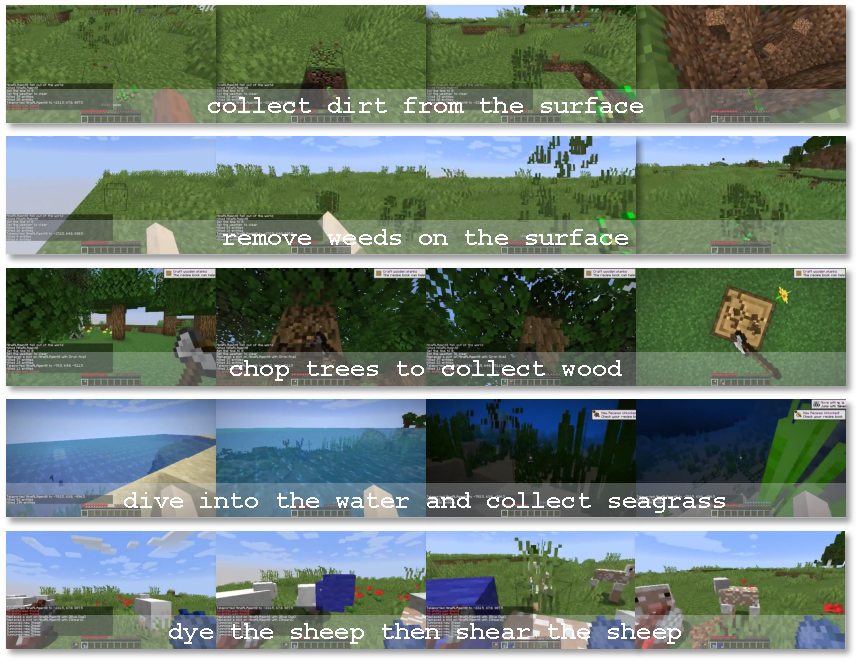
\includegraphics[scale = 0.9]{figures/benchmark_collect.pdf}
\end{center}
\caption{Examples of tasks in \texttt{collect} category. }
\end{figure*}


\definecolor{codeblue}{rgb}{0.25,0.5,0.5}
\definecolor{codekw}{rgb}{0.85, 0.18, 0.50}
\definecolor{keywordgreen}{rgb}{0,0.6,0}
\lstset{
  backgroundcolor=\color{gray!10},
  basicstyle=\fontsize{8pt}{9pt}\ttfamily\selectfont,
  columns=fullflexible,
  breaklines=true,
  captionpos=b,
  commentstyle=\fontsize{7.5pt}{7.5pt}\color{codeblue},
  keywords = {Task, Description, SkillAssessed, Evaluation, Precondition}, 
  keywordstyle = {\textbf},
  caption={The environment configuration and evaluation metric for \texttt{collect} series tasks. },
  label={lst:minecraft_deps_prompt}
}
\begin{lstlisting} % [language=python]  

Task: collect dirt
Description: Collect dirt from the surface. 
Precondition: Spawn the player in the plains biome. 
SkillAssessed: Basic terrain understanding and the ability to differentiate between surface-level blocks.
Evaluation: Run away. < Look down. < Dig down. < Break the dirt on the surface. 

Task: collect grass
Description: Remove weeds on the surface. 
Precondition: Spawn the player in the plains biome. 
SkillAssessed: Surface navigation and comprehension of vegetation blocks.
Evaluation: Run away. < Break the grass block. < Break a large field of grass blocks. 

Task: collect wood
Description: Cut down trees to collect wood. 
Precondition: Spawn the player in the forest biome with an iron_axe in its hand. 
SkillAssessed: Recognition of tree structures, efficient utilization of tools, and block harvesting capability.
Evaluation: Run away. < Approach trees. < Chop the tree and collect logs. 

Task: collect seagrass
Description: Dive into the water and collect seagrass. 
Precondition: Spawn the player near the sea. 
SkillAssessed: Water navigation, diving mechanics understanding, and underwater block interaction.
Evaluation: Walk on the land. < Swim on the water < Dive into the water. < Break seagrass blocks.

Task: collect wool
Description: Dye and shear the sheep for wool.
Precondition: Spawn the player in the plains biome with a shear (mainhand) and a stack of blue_dye (offhand), 5 sheep near the player. 
SkillAssessed: Interaction with entities, tool and item application, and sequential action execution. 
Evaluation: Ignore the sheep. < Dye the sheep. < Shear the sheep. < First dye then shear the sheep. 

\end{lstlisting}


